%%%%%%%%%%%%%%%%%%%%%%%%%%%%%%%%%%%%%%%%%
% University Assignment Title Page
% LaTeX Template
% Version 1.0 (27/12/12)
%
% This template has been downloaded from:
% http://www.LaTeXTemplates.com
%
% Original author:
% WikiBooks (http://en.wikibooks.org/wiki/LaTeX/Title_Creation)
%
% License:
% CC BY-NC-SA 3.0 (http://creativecommons.org/licenses/by-nc-sa/3.0/)
%
% Instructions for using this template:
% This title page is capable of being compiled as is. This is not useful for
% including it in another document. To do this, you have two options:
%
% 1) Copy/paste everything between \begin{document} and \end{document}
% starting at \begin{titlepage} and paste this into another LaTeX file where you
% want your title page.
% OR
% 2) Remove everything outside the \begin{titlepage} and \end{titlepage} and
% move this file to the same directory as the LaTeX file you wish to add it to.
% Then add \input{./title_page_1.tex} to your LaTeX file where you want your
% title page.
%
%%%%%%%%%%%%%%%%%%%%%%%%%%%%%%%%%%%%%%%%%

%----------------------------------------------------------------------------------------
%	PACKAGES AND OTHER DOCUMENT CONFIGURATIONS
%----------------------------------------------------------------------------------------

%Fixes pandoc tightlist error
\providecommand{\tightlist}{%
  \setlength{\itemsep}{0pt}\setlength{\parskip}{0pt}}

\documentclass[12pt]{article}
%\renewcommand{\familydefault}{\sfdefault}
\usepackage{amsfonts}
\usepackage{amssymb}
\usepackage{multicol}
\usepackage{graphicx}
\usepackage{titlesec}
\usepackage{longtable}
\usepackage{supertabular}

\usepackage{booktabs}
\setlength{\parindent}{0pt}
\setlength{\parskip}{1em}

\usepackage{hyperref}

%References

\usepackage[
backend=bibtex,
style=numeric,
autocite=footnote,
citestyle=authoryear
]{biblatex}

\addbibresource{references.bib}



\usepackage[british]{babel}
\usepackage{csquotes}

\usepackage{url}

\usepackage{microtype}


%	Below are optional commands to adjust the document.
%----------------------------------------------------------------------------------------
%----------------------------------------------------------------------------------------
%	Show's overfilled areas.
%----------------------------------------------------------------------------------------
%\overfullrule=2cm
%----------------------------------------------------------------------------------------

%----------------------------------------------------------------------------------------
%	Stop hyphenation.
%----------------------------------------------------------------------------------------
%\widowpenalty=10000
%\clubpenalty=10000
%----------------------------------------------------------------------------------------

%----------------------------------------------------------------------------------------
%	Adds a clear page after each section to start the next on a new page.
%----------------------------------------------------------------------------------------
%\newcommand\sectionbreak{\clearpage}
%----------------------------------------------------------------------------------------

%----------------------------------------------------------------------------------------
%	The following removes section numbering
%----------------------------------------------------------------------------------------
%\renewcommand{\thesection}{}
%\renewcommand{\thesubsection}{\arabic{section}.\arabic{subsection}}
%\makeatletter
%\def\@seccntformat#1{\csname #1ignore\expandafter\endcsname\csname the#1\endcsname\quad}
%\let\sectionignore\@gobbletwo
%\let\latex@numberline\numberline
%\def\numberline#1{\if\relax#1\relax\else\latex@numberline{#1}\fi}
%\makeatother
%----------------------------------------------------------------------------------------

\begin{document}

\begin{titlepage}

\newcommand{\HRule}{\rule{\linewidth}{0.5mm}} % Defines a new command for the horizontal lines, change thickness here

\center % Center everything on the page

%----------------------------------------------------------------------------------------
%	HEADING SECTIONS
%----------------------------------------------------------------------------------------

\textsc{\LARGE University of Brighton}\\[1.5cm] % Name of your university/college
\textsc{\Large Computer Science (Games)}\\[0.5cm] % Major heading such as course name
\textsc{\large Individual Project - CI301}\\[0.5cm] % Minor heading such as course title

%----------------------------------------------------------------------------------------
%	TITLE SECTION
%----------------------------------------------------------------------------------------

\HRule \\[0.4cm]
{ \huge \bfseries Final Year Project Report}\\[0.4cm] % Title of your document
\HRule \\[1.5cm]

%----------------------------------------------------------------------------------------
%	AUTHOR SECTION
%----------------------------------------------------------------------------------------

\begin{minipage}{0.4\textwidth}
\begin{flushleft} \large
\emph{Author:}\\
Adam \textsc{Worley} % Your name
\end{flushleft}
\end{minipage}
~
\begin{minipage}{0.4\textwidth}
\begin{flushright} \large
\emph{Supervisor:} \\
Marcus \textsc{Winter} % Supervisor's Name (Manos)
\end{flushright}
\end{minipage}\\[3cm]

% If you don't want a supervisor, uncomment the two lines below and remove the section above
%\Large \emph{Author:}\\
%John \textsc{Smith}\\[2cm] % Your name

%----------------------------------------------------------------------------------------
%	DATE SECTION
%----------------------------------------------------------------------------------------

{\large Hand in Date : 11\textsuperscript{th} of May 2017}\\[2cm] % Date, change the \today to a set date if you want to be precise

%----------------------------------------------------------------------------------------
%	LOGO SECTION
%----------------------------------------------------------------------------------------


\includegraphics[scale=0.60]{Images/BrightonLogo.jpg}\\[1cm] % Include a department/university logo - this will require the graphicx package

%\autocite{brightonlogo}


%----------------------------------------------------------------------------------------

\vfill % Fill the rest of the page with whitespace

\end{titlepage}
\tableofcontents
\pagebreak

\section{Methodology}\label{methodology}

A methodology is a set of methods, rules and restrictions combined to
form a procedure or discipline.

By adhering to a development methodology it is possible to set
development goals and a way to identify trouble areas during a project
allowing for plans and contingencies to be allocated to improve the
likelihood of success.

\subsection{Overview of types of
methodology}\label{overview-of-types-of-methodology}

There are many forms of methodologies, below are a few of the most
popular and an overview of each.

\subsubsection{Rapid Applications Development
(RAD)}\label{rapid-applications-development-rad}

By producing prototypes of the software quickly customers are able to
test and provide feedback as the software is developed. This is useful
as often requirements change and it's common for developers to produce
software that isn't actually what the customer wanted.

\subsubsection{Agile}\label{agile}

Originally project management was slow to adapt to changes with user
review coming in late stages of development. Agile however aims for
incremental development with regular feedback. \parencite{agile}

The most popular form of agile development is the Scrum
\parencite{agile} scrum is suited towards small teams and requires close
involvement by the product owner to provide regular feedback and review.

\subsubsection{Lean}\label{lean}

Much like scrum and other agile methodologies aims to produce software
quickly and involves close coordination with the product owner, where
lean varies is that it wants to reduce waste by selecting the most
valuable features required.\parencite{agilemethods}.

\subsubsection{Waterfall}\label{waterfall}

Focuses on phases such as; requirement gathering, analyses, development
and testing. Each phase is completed entirely before moving onto the
next phase and is often depicted by the phases flowing steadily
downwards resembling a waterfall.

\subsubsection{Spiral}\label{spiral}

The spiral model is based on the incremental model and consists of four
phases; Planning, risk analysis, engineering and evaluation
\parencite{spiral}. A project will go through each phase multiple times
in an iterative process or spirals. This is very well illustrated in the
figure below.

\begin{figure}
\centering
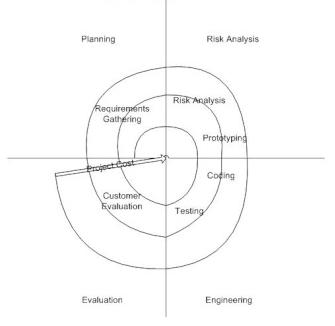
\includegraphics{../../Images/Spiral-model.jpg}
\caption{Spiral model diagram \parencite{spiral}}
\end{figure}

\subsubsection{Time Boxing}\label{time-boxing}

Involves strict deadlines rather than goals. By developing up to the
agreed upon time and evaluating progress this can allow for steadier
development and a set time in mind which provides a deadline for
development.

Evaluating at the end of the time frame can show struggles in the
development process and provides the ability to address them rather than
simply spending more time to complete the goal.

\subsection{Choice of methodology}\label{choice-of-methodology}

After assessing the various forms of project methodologies I have
decided to use an agile methodology most notably the Lean methodology as
this will provide me the ability to develop core functionality in a fast
pace and add other features time permitting. To assist my development I
will also be using time boxing to allocate time for my applications
functions and allow me to perform regular performance reviews so I can
identify time sinks and other issues to allow me to manage them.

\subsection{Project Time line}\label{project-time-line}

Below is a Gantt chart of the overall plan for my project. A Gantt chart
doesn't suit my development methodology very well and so is fairly
high-level overview.

\begin{landscape}
\begin{figure}[htbp]
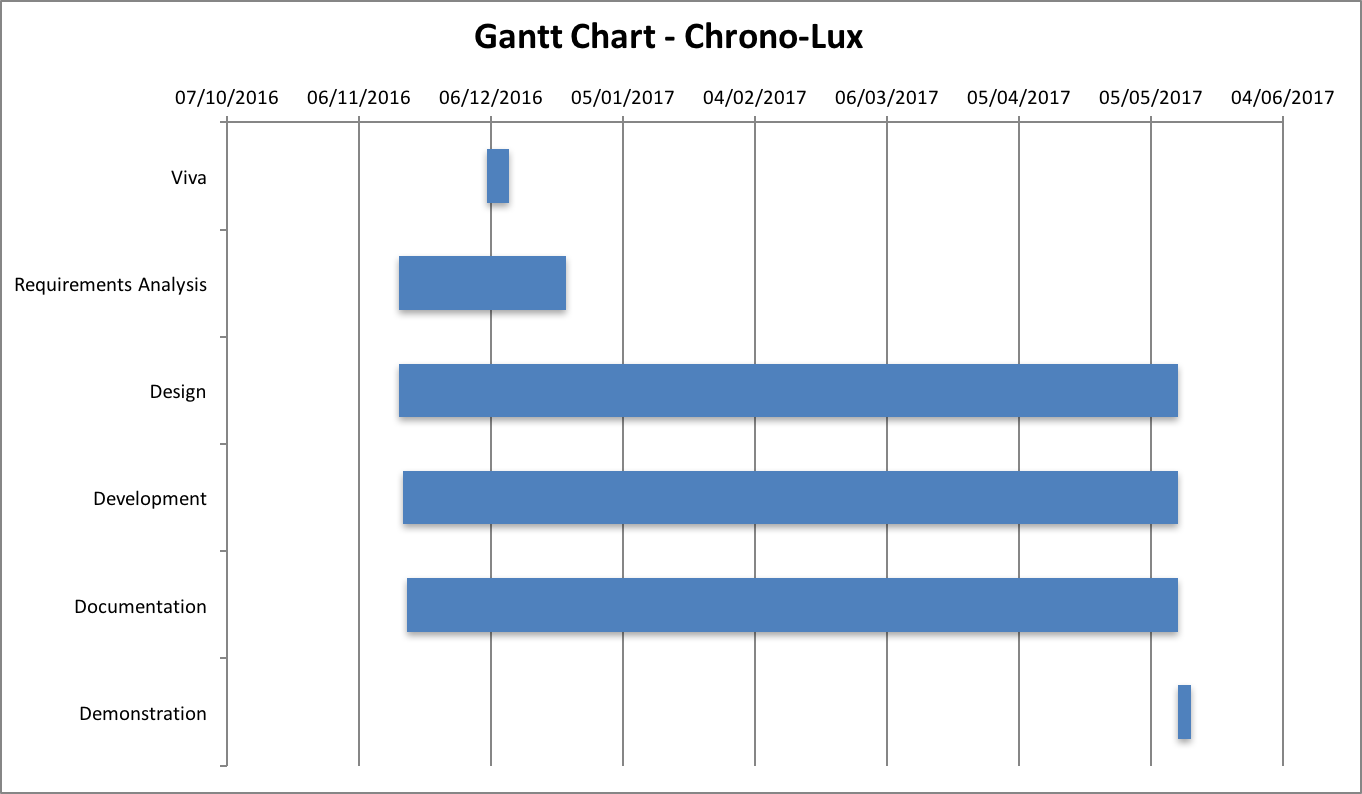
\includegraphics{Images/gantt.png}
\caption{Project Gantt Chart}
\end{figure}
\end{landscape}

\section{Stages of Development}\label{stages-of-development}

For a complete project there are fundamental stages that need to be
addressed, failure to address these stages can result in project drift
resulting in the end result not fulfilling expectations or failing to
achieve the requirements of the project.

It must be mentioned that although the term stages has been used, in
many methodologies especially those that involve rapid development many
of these stages will occur in either parallel or in quick succession;
for example testing will often happen throughout development to ensure
aspects of the code and design work as expected before extending the
software further.

\subsection{Analysis}\label{analysis}

The first stage of development is analysis, failing to analyse the
problem or obtain customer requirements renders development practically
impossible as the project scope can not be defined. Analysis often
requires the assessment of the problem or product to be developed and
rendering it down into more fundamental pieces such as how to implement
a RESTful API or store any data required. During this stage it is common
to perform competitor analysis by finding similar existing solutions to
challenges that may be faced and to implement improvements over the
competition and produce something objectively better to improve
usability, experience, performance and any combination of aspects that
can be deemed desirable.

\subsubsection{Competitors}\label{competitors}

\paragraph{\texorpdfstring{\href{http://sleep.urbandroid.org/}{Sleep as
Android}}{Sleep as Android}}\label{sleep-as-android}

This is the most feature packed alarm app available on Android that I
could find.

\subparagraph{Appearance}\label{appearance}

\begin{figure}[h]
  \begin{center}
    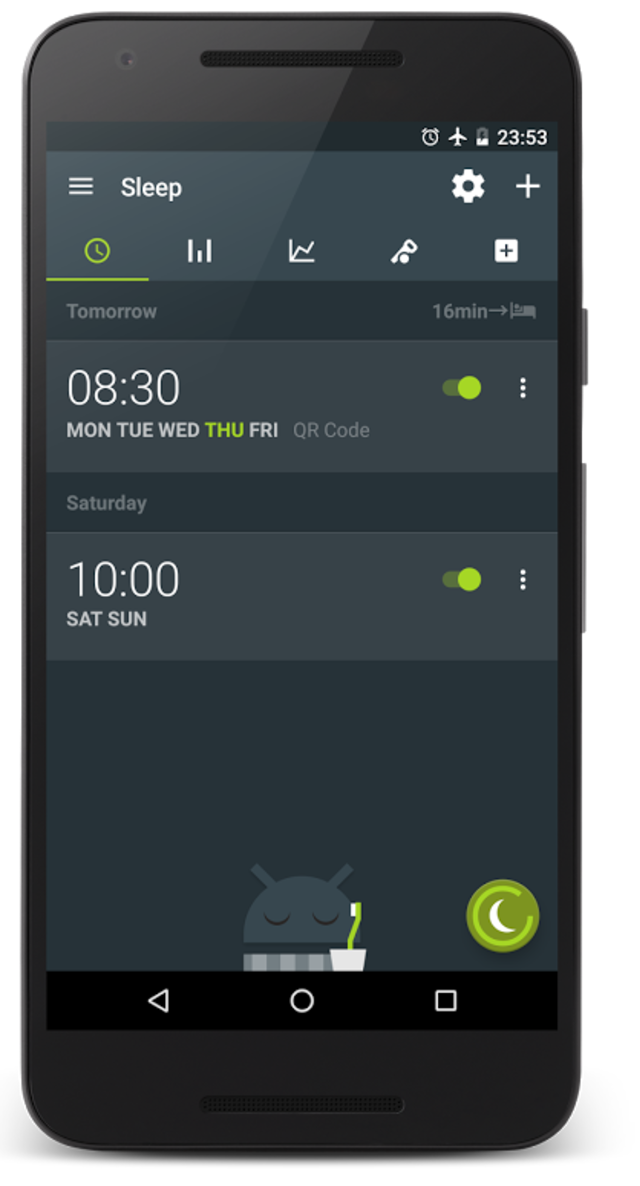
\includegraphics[scale=0.4,keepaspectratio]{Images/sleepas.png}
    \caption{Sleep as Android Screenshot}
  \end{center}
\end{figure}

The design of the app mostly follows the material guidelines set by the
Android development team with small variances in style. Overall the app
looks nice however some views can become crowded with information and
the number of features does make navigating the app harder than it needs
to be.

\subparagraph{Features}\label{features}

This app contains numerous features from the basics such as recurring
alarms to features such as solving a puzzle or scanning a QR code to
turn the alarm off. Features such as snore detection, sleep sensors and
sonar detection all detect and measure a persons sleep cycle and provide
statistics and graphs to assess the nights sleep and help inform the
user as how to improve their sleep quality, suggesting an earlier bed
time or to avoid sleeping aids and alcohol to prevent snoring.

\paragraph{\texorpdfstring{\href{https://cuckuu.com/}{Cuckuu}}{Cuckuu}}\label{cuckuu}

Cuckuu doesn't have the same level of integration with reminders,
appointments or weather as what I intend and it doesn't include any
smart bulb integration.

\subparagraph{Appearance}\label{appearance-1}

\begin{figure}
  \begin{center}
    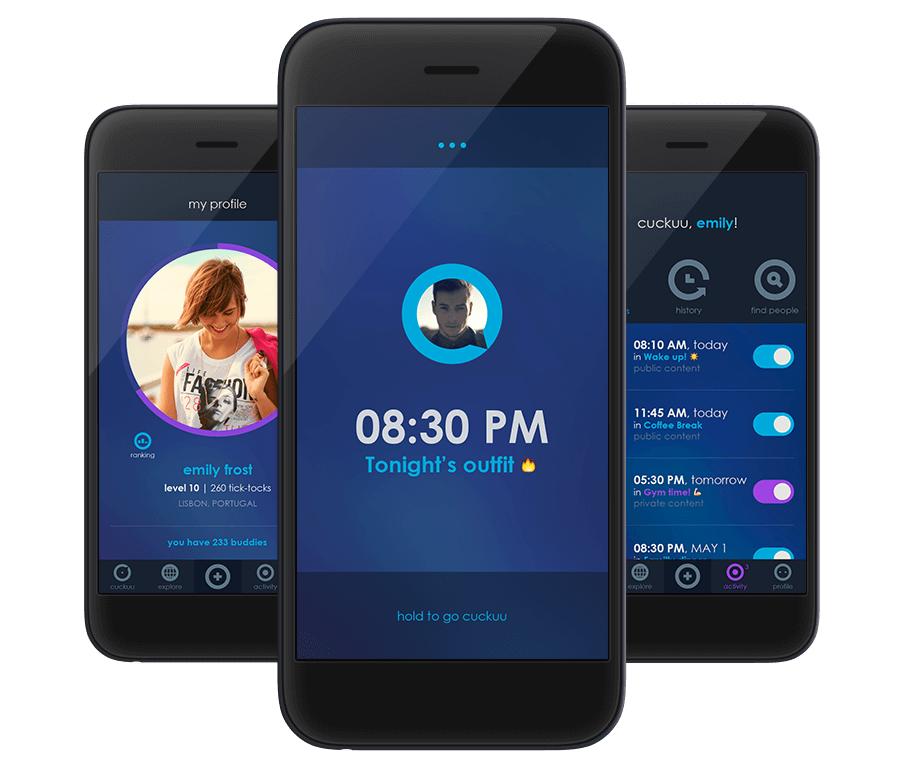
\includegraphics[scale=0.25,keepaspectratio]{Images/cuckuu.png}
    \caption{Cuckuu App Screenshots}
  \end{center}
\end{figure}

Cuckuu strikes a balance between Android and iOS allowing for it to be
available on both platforms, this is a good choice as it allows a user
to move between platforms and remain familiar with the design while
maintaining a good level of OS cohesion to keep the experience
consistent enough.

\subparagraph{Features}\label{features-1}

For Cuckuu social aspects of an alarm are the most important thing as
this is the apps unique selling point. Users are able to share alarms
(cuckuus) with their friends, possibly to alert them of shared events.

Users can add media or links to alarms both their own and shared alarms,
this provides a more visual and engaging alarm over a simple snooze and
off button. Another key aspect is a level of gamification towards alarms
by obtaining points for shutting of alarms quickly and providing a
leader-board among friends to encourage waking quickly and avoiding the
snooze button.

\paragraph{\texorpdfstring{\href{https://wakie.com/}{Wakie}}{Wakie}}\label{wakie}

Wakie is very different in how it intends to wake a user up and besides
being an alarm has little to what my app will consist of. Wakie does
have a very interesting concept though, that a stranger from around the
world will be able to call you when you would like to be woken and talk
about a topic you would like to discuss.

\paragraph{Appearance}\label{appearance-2}

\begin{figure}[htbp]
\centering
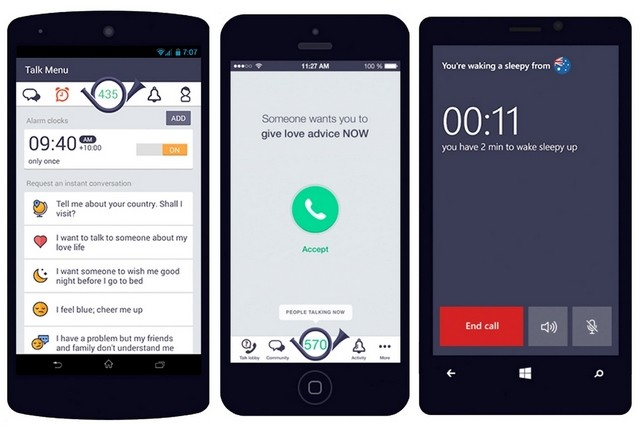
\includegraphics{Images/wakie.jpg}
\caption{Wakie App}
\end{figure}

With a very simple and clean design this app definitely looks nice and
allows itself to easily be ported into the varying mobile platforms.

\paragraph{Features}\label{features-2}

Since the initial analysis of this application the alarm aspects have
since been removed, as such I will be writing about the app in regards
to older versions that still contained the alarm functionality.

Overall the app works simply, you can set an alarm and another user of
the app will be connected to you through a phone call at the time the
alarm is set for. The concept is to provide a more sociable and personal
alarm, knowing that your alarm is a person on the other end possibly
encourages the user to wake up more than a simple alarm. The app and
it's functionality are free and only users of the app are connected
together.

\subsubsection{Problem Analysis}\label{problem-analysis}

Through my competitor analysis it is clear there is little competition
for smart-device connected alarm applications and with the increase in
smart-device popularity I feel there is a market for such an
application. The problems with existing alarm applications can be
attributed to their functionality, in some cases the amount of
functionality can be overwhelming in the case of \emph{Sleep as Android}
I feel there are just far to many features and this produces are
cluttered experience.

By focusing on a small amount of features such as how Wakie focuses on
an alarm with a chat, I intend to make a clean and simple app that is
familiar to the material design guidelines for the Android platform to
make my app blend seamlessly.

\subsection{Design}\label{design}

During the design stage the User Interface (UI) and various aspects of
the code are planned for development. By critically thinking about
certain design aspects with regards to the requirements outlined from
the analysis stage, designs of the software can be produced, this
includes both the visual designs of the user interface and some of the
software solutions that may be required such as certain tooling and
frameworks that are available for development to produce more stable
software faster by removing the need to produce custom solutions to
aspects that have been solved and are found throughout programming.

\subsubsection{Design Considerations}\label{design-considerations}

The application will often be used within a low-light or dark scenario
and as such I will design the application to use a dark colour scheme.

A light colour scheme could be quite energising to the user and could
potentially make them more alert which is not ideal before going to
sleep and could extend the duration it takes to fall asleep, resulting
in restlessness.

It has been shown blue light in particular can affect the circadian
rhythm of the body which is used to regulate sleep patterns
\cite{oh2015analysis}.

\subsubsection{Designs}\label{designs}

\emph{TODO} APPENDIX?

\subsection{Development}\label{development}

Throughout development everything that has been produced from both the
analysis and design stages are implemented through creation and
utilisation of software and assets such as images and sounds to produce
the goal of the project, in the instance of a mobile application this
would consist of producing and application that can run on the required
platforms such as Android, iOS or Windows Phone and for the application
to perform the tasks required such as sending and receiving messages and
displaying them to the user in the case of a communications application.

\subsubsection{Platform}\label{platform}

The development platform chosen is for Android devices, this is due to
the lead market share of mobile devices and through the relatively
simple and free development platform using Android studio and the
Android Virtual Device (AVD) tools provided, with the AVD providing the
ability to test applications on every version of Android available and
with different device specifications such as screen size, screen
density, on-board sensors and orientations.

With my personal phone being an Android device it is also possible to
install, test and debug my application on a physical device which is
often faster than a virtual device and can provide a better experience
of what the application will be when deployed.

\subsubsection{Target Market}\label{target-market}

Through various factors including my chosen platform, I will be
targeting the latest version of the Android platform 25 also known as
Nougat with support for devices as old as version 21 known as Lollipop.
My decision is based on the current version distribution statistics that
show over 50\% of devices are on versions 21 or higher and as such my
target is the majority share.

Version 19 (KitKat) currently hold a 20\% share which is a large
portion, however these are older devices that are likely to be from
poorer markets and due to the cost of smart-devices it is unlikely for
there to be a high demand of support from my app for KitKat. Due to the
release and support cycle provided by Google it is also likely for
KitKat to be unsupported by the end of the year and as such I feel there
are greater benefits to gain from the newer versions in place of using
older development features and supporting deprecated code.

Due to time limitations support will only be provided in English, with
the app having no alternative language support. From the restrictions
and targeted versions I will be focusing on countries that have English
as the native speaking language and areas of relative wealth as these
are the most likely to have access to the required smart-devices.

\subsection{Testing}\label{testing}

Often testing is an ongoing aspect of the development life cycle so that
as aspects of the application are developed tests and unit testing
classes are produced to allow the automation of testing. Performing
ongoing testing is useful to indicate that code is working correctly and
if during development if the automated testing indicates any issues
these can be resolved as they occur instead of during feedback or after
deployment, both of which increase development cost through having to
hunt down bugs and maintain the application during the life time of the
application.

\subsubsection{Tests}\label{tests}

The majority of testing involved will consist of introducing
functionality into the app and performing various actions to test that
functionality by using it as intended and trying to break it through
fringe cases and interactions that are likely to be less common such as
rapidly editing a text input or using input that is likely to be
uncommon such as number in place of text.

Further testing in the later stages of development will use others to
use the app and to provide feedback for their experience. It is very
difficult to test all cases as issues with UI or networking can be
intermittent and as such development should involve writing good code
and be less reliant on tests to indicate when something isn't working.

\subsection{Feedback}\label{feedback}

Feedback is crucial for assessing the success of a project, by obtaining
feedback from testers or trial users changes can be made to improve the
experience of the application. Feedback can be obtained during
development by having people use certain aspects of the application as
it's being developed. If during feedback multiple users raise complaints
about the same aspects this is a key indicator to change that aspect of
the application before full deployment to ensure a higher level of
polish and maintain a higher level of respect and image.

\subsubsection{User Trials}\label{user-trials}

As mentioned later stages of testing will involve others to test my app,
through testing I can obtain feedback for the design, usability and
highlight issues that I may not have accounted for in my development and
testing.

\section{Accomplishments}\label{accomplishments}

The following are some of the accomplishments within developing my
application of which I am most proud.

\subsection{The Ability to Control
Lighting}\label{the-ability-to-control-lighting}

There are few applications available that allow for the connection to
and manipulation of smart-lights from within the application. Because of
my app being one of these I feel is an accomplishment.

\subsection{The Application UI Design}\label{the-application-ui-design}

Overall I feel the look and feel of my application works very well; it
adheres to the Android design guidelines \parencite{androiddesign} and
feels like a native application by maintaining a cohesive user
experience.

\subsubsection{Tab Navigation}\label{tab-navigation}

The tab navigation works well, providing the user with a simple and
clean way for using my application. By providing only the relevant
functionality for each tab the user experience is simple and intuitive.
Through avoiding too much being displayed on the screen at once,
relevant information can be seen instantly ensuring ease of use and
allowing the user to only spend as long as necessary within the
application.

Through including tab navigation it was required to use fragments within
my application, fragments are not as simple to use as a regular activity
and pose multiple design challenges over an application activity. The
extra difficulty associated with fragments did slow the initial
development of my application and my initial tab view needed to be
replaced due to the use of several deprecated styles. Despite this
challenge I feel the fragments work well within my application and the
functionality I outlined within my project has been accomplished.

\subsubsection{Snackbars and Toasts}\label{snackbars-and-toasts}

By developing for newer versions of Android I utilised the snackbar
notification system introduced in API level 23. The snackbar in most
instances replaces the original Toast notification system. Snackbars
improve upon toast in many ways as they; provide information to the user
and allow the user to interact with the notification by performing an
action if provided by the snackbar, such as undoing an action that
triggered the snackbar to be displayed. The snackbar can also be
dismissed by swiping, while the toast is displayed until the specified
display time has passed.

Toasts are stilled used within the newer versions of Android, however
they are now often used for system notification as they can be displayed
without being associated with an activity and as they can't be dismissed
are good for showing warnings or important information. Snackbars also
blend better within an application, showing up above or moving elements
such as a floating action button, ensuring that the notification can be
seen and that aspects of the view are not obstructed.

It is specified within the guidelines that a snackbar should be
displayed as long as necessary, as such short notifications should not
be displayed for a long time, while notifications that provide an action
or consist of a lot of text should be displayed for longer to allow the
user to fully read the text or provide adequate time for interaction.

\subsubsection{Using the Weather Icon
Font}\label{using-the-weather-icon-font}

The usage of the weather icon font provides multiple advantages over
that of PNG, JPG or SVG graphics. Of these graphics types JPG doesn't
allow for transparency and so would require a background colour to be
saved, this would not only increase the storage space required to store
the image, but would require the image to be edited if the background
colour of the view were to be changed, making the use of a stored
background difficult to manage. PNG does allow for transparency, however
PNG images requires a relatively larger amount of storage space when
compared with JPG.

PNG and JPG are bitmap image types, meaning they store all the pixel
data such as colour values and luminosity among other values as
essentially a three dimensional array over the colour space. Due to the
means of storage the graphics are not suitable for scaling, especially
to increase the size of the graphic as this would require the need to
generate data that does not exist; for example in an image that is
\(800 \times 800\) pixels, there would be 640,000 pixels, if the image
were scaled to \(1000 \times 1000\) pixels there would need to be
1,000,000 pixels and as a result 360,000 pixels need to be generated
from the existing image, resulting in processing artefacts, banding or
other graphical errors.

SVG is a vector graphic and consists of instructions on how to draw a
graphic and this is handled when the image is to be displayed. Due to
this flexible drawing ability, the graphic can be generated to be as
large as required with a trade off of computational time for storage,
compared to bitmap images. Android is now capable of handling both
types, however this has not always been the case. SVG support has been
officially supported for versions above 4.4 (KitKat) with many adopting
workarounds using the webview library prior to support
\parencite{svgAndroid}. As a result there are many poor implementations
of using SVG and the current advice provided in the Android guidelines
is to generate PNG graphics from SVG files as to support older devices.
When the PNG files are produced multiple sizes can be generated to
support devices of varying screen sizes and in doing so requires
multiple sizes of the same file to be saved, taking up more storage
space.

By using a TrueType Font (TTF) it is possible to gain the benefits of an
SVG without the need to generate resource files or use unsupported
implementations to display the graphics. Other benefits include the
ability to easily colour the icons by changing the font colour, the font
appears as a single file within the Android project resulting in less
clutter in the project structure. Lastly the size required to store the
font consisting of hundreds of icons is relatively small as it requires
98kb of storage while a single large PNG around 30kb.

\section{Research}\label{research}

There are aspects of my project that my research before and during
development influenced my app from what I had initially planned.

\subsection{Philips Hue API}\label{philips-hue-api}

My project utilises the Philips Hue connected light bulbs, the
\cite{philipshue} system uses the \cite{zigbee} standard, though all of
this is transparent as the method of interfacing with the devices is to
use `GET', `PUSH', `POST' and `PUT' URL requests and provide JSON
formatted commands in the body to interact.

The state of a specific light can be received using `GET' and providing
the URL /api/devID/lights/1 or all of the lights by not specifying the
number.

The state can be changed using `PUT' instead and providing attributes
and their values that you would like to change, for example:

\begin{lstlisting}
{"on":true, "bri":255}
\end{lstlisting}

A few useful attributes for my application are: on = true/false bri =
Brightness between 0 and 254

Colour settings include: sat = Saturation between 0 and 254 hue = The
hue of the light (hue runs from 0 to 65535)

Through researching into the Hue API further there existed a Hue
Software Development Kit (SDK), by using implementation of the Hue SDK
most interactions with the lighting that would require the use of the
RESTful API are now able to be accessed using Java methods. The Hue SDK
exists alongside a very basic example Android application that allows
the connection to the Hue bridge used for interfacing with the lights
and a button to randomly adjust the hue values of the lights connected
to the bridge.

\subsubsection{Influence}\label{influence}

The implementation example of the bridge connection and the storage of
the API key required to authenticate a connected device/application
included was very useful for the initial set-up for interfacing with the
Hue lighting platform and as such a direct use of the RESTful API has
not been implemented within my application to interface with the Hue
lighting but instead the Hue SDK.

\subsection{Design Considerations}\label{design-considerations}

Through my research I have found that it has been shown bright lighting,
blue light in particular can affect the circadian rhythm of the body
which is used to regulate sleep patterns \cite{oh2015analysis}. There
are applications used to reduce the amount of blue light displayed in
the evening and through the night, applications such as flux
\parencite{flux} and features included within mobile operating systems
such as iOS \parencite{iosNightShift} and Android platforms
\parencite{samsungBlueFilter}.

\subsubsection{Influence}\label{influence-1}

My application will often be used within a low-light or dark scenario
and as such I will design the application to use a dark colour scheme.

A light colour scheme could be quite energising to the user and could
potentially make them more alert which is not ideal before going to
sleep and could extend the duration it takes to fall asleep, resulting
in restlessness and a poor nights sleeps.

\subsection{Human Perception of Light}\label{human-perception-of-light}

Many human senses are based on a logarithmic scale, this is to say we
are far more able to distinguish changes in light or sound in the lower
band of the senses compared to higher, as such a small increase in
volume of a whisper will be a more distinguishable change in volume than
two jet engines roaring and increasing by their volume by a small
amount.

The same applies to sight, it is more important to distinguish details
in low light such as that from the moon compared to the light change of
daylight at varying times of the day. We do this to normalise our senses
to best suit our environment.

This kind of stimulus perception is defined as the just-noticeable
difference (JND). Firs summarised by Ernst Weber in 1834 his equation
was called Weber's Law and simply stated that response intensity
increases as stimulus intensity increases
\parencite[p. 1613-1615]{salkind2010encyclopedia}. Further refined by
Gustav Fechner who proposed the use a constant to provide a curve to the
stimulus/perception relationship. Fechners' law was a much better fit,
however some stimulus did not fit well, such as that of electric shock.

Most recently in the 60's an American psychologist S. S. Stevens
produced a formula that worked for all forms of stimulus, even for
electric shocks \parencite{stevens1957psychophysical}. He proposed an
exponential function raising the data to a power rather than using a
simple constant. This essentially stated that to get a linear increase
in perception of various stimuli, the stimulus would need to increase in
an exponential form.

\subsubsection{Influence}\label{influence-2}

Due to this perception of light I feel increasing the brightness of the
lighting in the room in a logarithmic fashion will produce a perceptibly
more natural and linear increase in brightness over increasing the value
directly from 0 to the maximum value.

\section{Success and Failure}\label{success-and-failure}

In this section is an assessment of some of the successes or failures of
the project as a whole.

\subsection{Successes}\label{successes}

Within the project there were some highlights of success that are
mentioned as follows.

\subsubsection{The Project}\label{the-project}

As outlined within the project specification several goals and stretch
goals were set and if the goals were meant this would regard the project
as being a success. The application provides; alarm functionality, smart
bulb integration and weather functionality each of which are the main
goals set and as such the project was a success.

\subsubsection{Using SQLite}\label{using-sqlite}

I had not foreseen the need to use a database within my application as
the storage of alarms had not seemed to be a complex enough scenario to
need a database. As the other storage methods available were not suited
for storing an object with multiple variables however it was necessary
to utilise the SQLite database for storage.

Though more complex than other storage methods, the use of database
helpers reduced the need to write raw SQL queries and requests and
allowed for a more programmatic style to interface with the database.
Overall the database worked well.

\subsubsection{Pending intents}\label{pending-intents}

When developing the alarm and using the alarm manager it was necessary
to use pending intents. Pending intents are simple enough to understand
however their implementation is a little odd, as cancelling a pending
intent requires another matching pending intent being produced, however
the use of the \lstinline!cancel()! method at the end cancels the
pending intent.

Due to this and the need to allow the user to enable and disable an
alarm, it was necessary to leave the pending intent and instead to check
the alarm that was being triggered was enabled. In doing so there is no
longer a need to create and delete pending intents for alarms that had
been disabled, as the alarm object would still exist within the database
and could cause errors if there was an ID mismatch.

\subsection{Failures}\label{failures}

Although the project was successful, there are several aspects that
failed to be implemented or did not make it into the final application.

\subsubsection{No Adjustable alarm}\label{no-adjustable-alarm}

Due to the time picker not returning values, the alarms are created from
within the listener method, because of this it made it difficult to be
able to allow for alarms to be changed once set. The lack of ability to
pass values into the time picker means that there is no way to pass an
alarm id into the method either, something that could allow for a check
to see if an alarm by that ID already exists, if the alarm does exist
adjust the time and if not create a new alarm.

\subsubsection{Not Reaching Stretch
Goals}\label{not-reaching-stretch-goals}

This could be classed as not being a failure, as the main goals outlined
have been met. However I feel that the stretch goals would have worked
well within my application and helped it to stand out more through being
more than a regular alarm application, more so than the inclusion of
controlling smart-lights.

\section{Assessment of Progress}\label{assessment-of-progress}

an assessment of the progress you made, problems encountered, their
solutions and the lessons learned

\subsection{Progress Made}\label{progress-made}

\subsection{Problems Encountered}\label{problems-encountered}

\subsubsection{Alarm creation}\label{alarm-creation}

\paragraph{Solution}\label{solution}

\subsubsection{Storing Objects}\label{storing-objects}

\paragraph{Solution}\label{solution-1}

\subsection{Lessons Learned}\label{lessons-learned}

\section{Further Areas of Investigation and
Enhancements}\label{further-areas-of-investigation-and-enhancements}

\subsection{Further Investigation}\label{further-investigation}

\subsection{Enhancements}\label{enhancements}

Other smart-devices not just lights.

\section{Original Plan}\label{original-plan}

Include your original project plan, together with any later versions or
a discussion of any necessary changes to the plan. We recommend a count
of 5000 words. This report is an assessable component of the project and
is one the examiners will pay close attention to. Please hand in one
copy by 18th May 2017. All reports MUST contain a first page with
student name, student number, exit award for which you are registered
and a short title.

\section{Evaluation}\label{evaluation}

The following is a critical evaluation of every significant area my
project, including my choice of project and how it fits in with the
modules that I have studied over the course of my degree.

\subsection{Choice of Project}\label{choice-of-project}

Deciding upon a project that was challenging and feasible for the amount
of time allocated for completion was quite a difficult task. Many ideas
and concepts that I thought of were either already well investigated or
posed the risk of being incomplete by the final deadline. I proposed
several ideas for a final year project to Marcus Winter, my project
supervisor and he helped me decide upon my home automation alarm as the
project that I should undertake.

The project I decided upon however addressed less of a computer science
research project and instead is more focused on user design and
interaction.

My reasons for the choice of my project are due to my interest in mobile
applications development and in the concept of home automation. I'm
particularly interested in a future in which many common actions are
handled transparently by automated systems, such as opening and closing
curtains and adjusting lighting as required by the user without the need
for direct user interaction and many other situations that can provide
benefits by saving time each day, to assisting those who are unable to
live alone and require regular assistance and house calls.

Overall I feel the project I chose has been challenging and is suited
towards my degree

\subsection{Course Relation}\label{course-relation}

Over the course of my degree I have undertaken multiple modules many of
which are relevant to my final project.

\subsubsection{Mobile Application
Development}\label{mobile-application-development}

Mobile app development is one module that clearly relates to my final
year project having worked on a mobile application for my project.
Throughout the module issues such as platform independent issues and
general principles for mobile user interaction design and the
constraints of developing for a mobile platform.

The issues surrounding mobile web vs native applications were also
addressed, deciding on leveraging native tools by developing directly
for a platform or for the development of a cross platform application.

There are also many platform specific issues from the development
environment and tool-chain, to the architecture and APIs provided that
need to be addressed throughout the development and maintaining of the
application.

I have worked with both physical and virtual devices and have been able
to see the benefits and restrictions of both, such as leveraging the
speed of a physical device both in installation and application usage,
over the ability to emulate numerous devices and test the application in
ways that could be very costly and time consuming.

Many requirements of most applications today are the need for;
persistence and storage, multimedia, interacting with hardware sensors
and web services. Arguably most important of all the deployment to the
relevant platforms application store was also addressed, allowing an
application to go from a development build to a signed and globally
installable application.

\subsubsection{Programming languages, concurrency and client server
computing}\label{programming-languages-concurrency-and-client-server-computing}

As Android is based upon the Java development language

Java

UI thread and concurrency

RESTful

\subsubsection{Project management}\label{project-management}

\subsubsection{User design and product
evaluation}\label{user-design-and-product-evaluation}


\pagebreak
\printbibliography

All links were last followed on the 9\textsuperscript{th} of November, 2016

\end{document}
